\documentclass[a4paper]{article}
\usepackage[english]{babel}

% Mathematical notation and symbols
\usepackage{amsmath}
\usepackage{amsfonts}
\usepackage{amssymb}
\usepackage{bbold}

% Figures and hyperlinks
\usepackage{graphicx}
\usepackage[hidelinks]{hyperref}

% Theorem environments
\usepackage{amsthm}
\newtheorem{theorem}{Theorem}
\newtheorem{lemma}{Lemma}

% Use the figures stored with the original report
\graphicspath{{../report/}}

\begin{document}
\pagenumbering{arabic}

\Large
\begin{center}
Assignment 3\\

\hspace{10pt}

% Author name and affiliation
\large
Julio A. Medina$^1$ \\
\hspace{10pt}
\small
$^1$ University of San Carlos\\
School of Physical and Mathematical Sciences\\
Master's Degree in Physics\\
\href{mailto:julioantonio.medina@gmail.com}{julioantonio.medina@gmail.com}\\
\end{center}

\hspace{10pt}

\normalsize
\section{Initial Value Problem}

Solve the following initial value problem:

\begin{equation}
y''-2xy'-y=y^2 e^{-x^2}.
\end{equation}

The initial conditions are

\begin{equation*}
y(0)=1,\qquad y'(0)=0.
\end{equation*}

Use two steps of the Runge--Kutta method, as described in \cite{Burden}, with $h=0.5$ and $h=0.25$.

A C program was implemented to solve this initial value problem. The source code is available at \url{https://github.com/Julio-Medina/Runge-Kutta/tree/main/code}.

\begin{figure}[h]
\centering
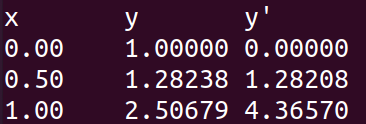
\includegraphics[scale=0.4]{rkh05.png}
\caption{RK4 result with $h=0.5$.}
\label{fig:rk4-h05}
\end{figure}

\begin{figure}[h]
\centering
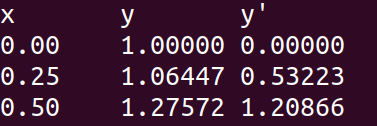
\includegraphics[scale=0.4]{rkh025.png}
\caption{RK4 result with $h=0.25$.}
\label{fig:rk4-h025}
\end{figure}

\begin{thebibliography}{99}

\bibitem{Burden}
Richard L. Burden and J. Douglas Faires,
\textit{Numerical Analysis}, 9th ed.,
Brooks/Cole, Cengage Learning.
ISBN 978-0-538-73351-9.

\end{thebibliography}
\end{document}
